\chapter{Power Management IC Compatibility}
\label{ch:pmic}

\section{Overview}
\label{sec:pmic_overview}

This chapter looks beyond the rectifier stage studied throughout the rest of the thesis, to the power management integrated circuit (PMIC) that would sit downstream of it in a complete energy-harvesting system, converting the rectified output into a regulated supply for the load. Since three different rectifier topologies were built and characterised (the star and delta connections of the FWR, and the NVC), each presents a downstream PMIC with a different open-circuit voltage as a function of rotational speed. Section \ref{sec:pmic_ocv} reports this voltage for all three topologies, Section \ref{sec:pmic_candidates} introduces five commercially available PMICs suited to sub-watt harvesting sources, and Section \ref{sec:pmic_compatibility} compares the two to identify which topology-PMIC pairings are electrically compatible, and at which speeds, over the tested range.

\section{Open-Circuit Voltage Across Topologies}
\label{sec:pmic_ocv}

Tables \ref{tab:pmic_ocv_star}-\ref{tab:pmic_ocv_nvc} report the open-circuit voltage $V_{OC}$ measured at the output of each rectifier topology, i.e.\ with no load connected ($R_L=\infty$), together with the high-frequency ripple superimposed on it, over the same $100$-$400\ \text{rpm}$ speed range used throughout Chapter \ref{ch:measurements}. This is the voltage a downstream PMIC's input pin would see before any load is drawn, and is the quantity compared against each candidate PMIC's input voltage range in Section \ref{sec:pmic_compatibility}.

\begin{table}[htbp]
    \centering
    \begin{tabular}{ccc}
        \toprule
        Speed (rpm) & $V_{OC}$ (V) & Ripple (V) \\
        \midrule
        100 & 1.98 & 0.012 \\
        150 & 2.83 & 0.012 \\
        200 & 3.67 & 0.011 \\
        250 & 4.51 & 0.012 \\
        300 & 5.32 & 0.012 \\
        350 & 6.17 & 0.011 \\
        400 & 7.04 & 0.012 \\
        \bottomrule
    \end{tabular}
    \caption{Open-circuit voltage of the FWR star connection.}
    \label{tab:pmic_ocv_star}
\end{table}

\begin{table}[htbp]
    \centering
    \begin{tabular}{ccc}
        \toprule
        Speed (rpm) & $V_{OC}$ (V) & Ripple (V) \\
        \midrule
        100 & 1.000 & 0.022 \\
        150 & 1.460 & 0.021 \\
        200 & 1.910 & 0.017 \\
        250 & 2.365 & 0.017 \\
        300 & 2.825 & 0.017 \\
        350 & 3.275 & 0.017 \\
        400 & 3.755 & 0.017 \\
        \bottomrule
    \end{tabular}
    \caption{Open-circuit voltage of the FWR delta connection.}
    \label{tab:pmic_ocv_delta}
\end{table}

\begin{table}[htbp]
    \centering
    \begin{tabular}{ccc}
        \toprule
        Speed (rpm) & $V_{OC}$ (V) & Ripple (V) \\
        \midrule
        100 & 2.70 & 0.547 \\
        150 & 3.05 & 0.691 \\
        200 & 3.20 & 0.639 \\
        250 & 3.15 & 0.566 \\
        300 & 3.15 & 0.476 \\
        350 & 3.15 & 0.414 \\
        400 & 3.15 & 0.369 \\
        \bottomrule
    \end{tabular}
    \caption{Open-circuit voltage of the NVC.}
    \label{tab:pmic_ocv_nvc}
\end{table}

The star connection's open-circuit voltage grows the most steeply with speed, from $1.98\ \text{V}$ at $100\ \text{rpm}$ to $7.04\ \text{V}$ at $400\ \text{rpm}$, consistent with the highest output power found for this connection in Chapters \ref{ch:measurements} and \ref{ch:comparison}. The delta connection's open-circuit voltage grows over the same range but stays well below the star connection's at every speed, from $1.00\ \text{V}$ to $3.755\ \text{V}$. The NVC's open-circuit voltage instead rises only up to $200\ \text{rpm}$, where it peaks at $3.20\ \text{V}$, and settles to $3.15\ \text{V}$ for every higher speed tested; its ripple is also an order of magnitude larger than either FWR connection's, consistent with its active, switching mode of operation described in Section \ref{sec:nvc}.

\section{Candidate Power Management ICs}
\label{sec:pmic_candidates}

This section summarises five commercially available PMICs considered as candidates for the six-phase harvester, each specified in terms of the input voltage range it accepts from the rectifier stage and the outputs it regulates that range down to.

\subsection{DS-AEM13920\_VR}
\label{sec:pmic_aem13920}

\href{https://e-peas.com/documents/AEM13920/DS-AEM13920.pdf}{Datasheet} \cite{epeasAem13920Datasheet}

\begin{figure}[htbp]
    \centering
    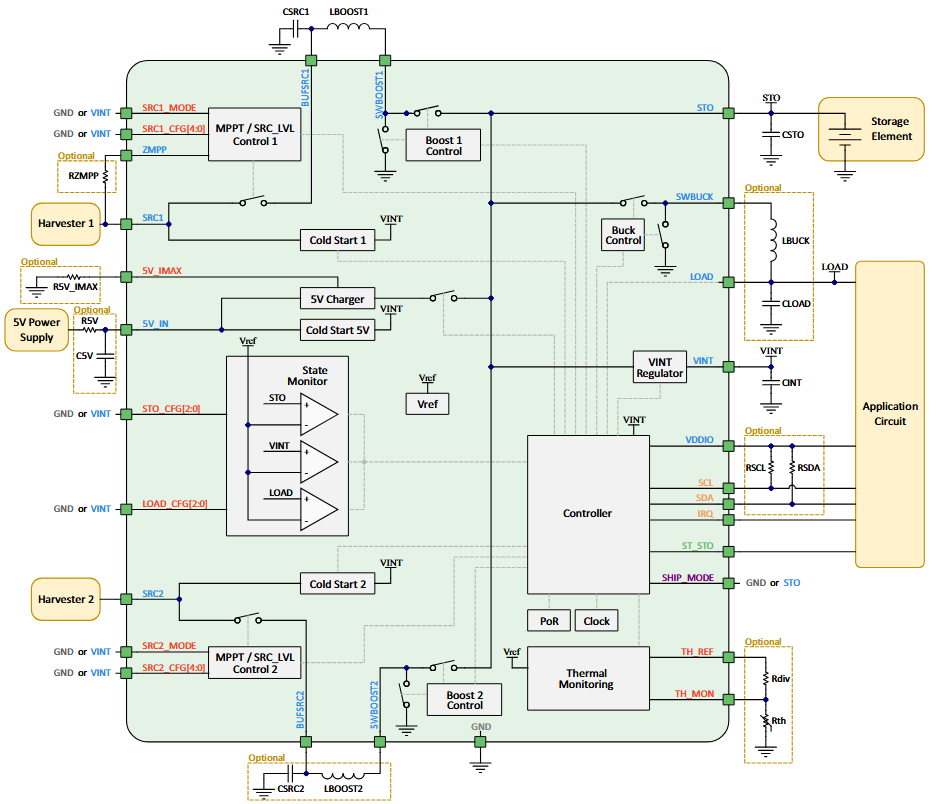
\includegraphics[width=0.65\textwidth]{imm/DS-AEM13920_VR_Block_Diagram.png}
    \caption{DS-AEM13920\_VR block diagram.}
    \label{fig:pmic_aem13920}
\end{figure}

\begin{table}[htbp]
    \centering
    \begin{tabular}{cccc}
        \toprule
        Symbol & Parameter & Range & Unit \\
        \midrule
        $V_{in}$ & Source input voltage & $0.120$-$4.6$ & V \\
        $V_{cs}$ & Source cold-start voltage & $0.275$ & V \\
        $V_{OC}$ & Open-circuit voltage tracked for MPP & $0$-$5$ & V \\
        \bottomrule
    \end{tabular}
    \caption{DS-AEM13920\_VR input stage.}
    \label{tab:pmic_aem13920_in}
\end{table}

The output voltage is regulated with a Buck converter connected to the storage element.

\begin{table}[htbp]
    \centering
    \begin{tabular}{cccc}
        \toprule
        Symbol & Parameter & Range & Unit \\
        \midrule
        $V_\text{Buck}$ & Buck output voltage & $0.6$-$2.5$ & V \\
        $I_\text{Buck}$ & Buck output current & $0$-$100$ & mA \\
        \bottomrule
    \end{tabular}
    \caption{DS-AEM13920\_VR output stage.}
    \label{tab:pmic_aem13920_out}
\end{table}

\subsection{DS-AEM10941\_VR}
\label{sec:pmic_aem10941}

\href{https://e-peas.com/documents/AEM10941/DS-AEM10941.pdf}{Datasheet} \cite{epeasAem10941Datasheet}

\begin{figure}[htbp]
    \centering
    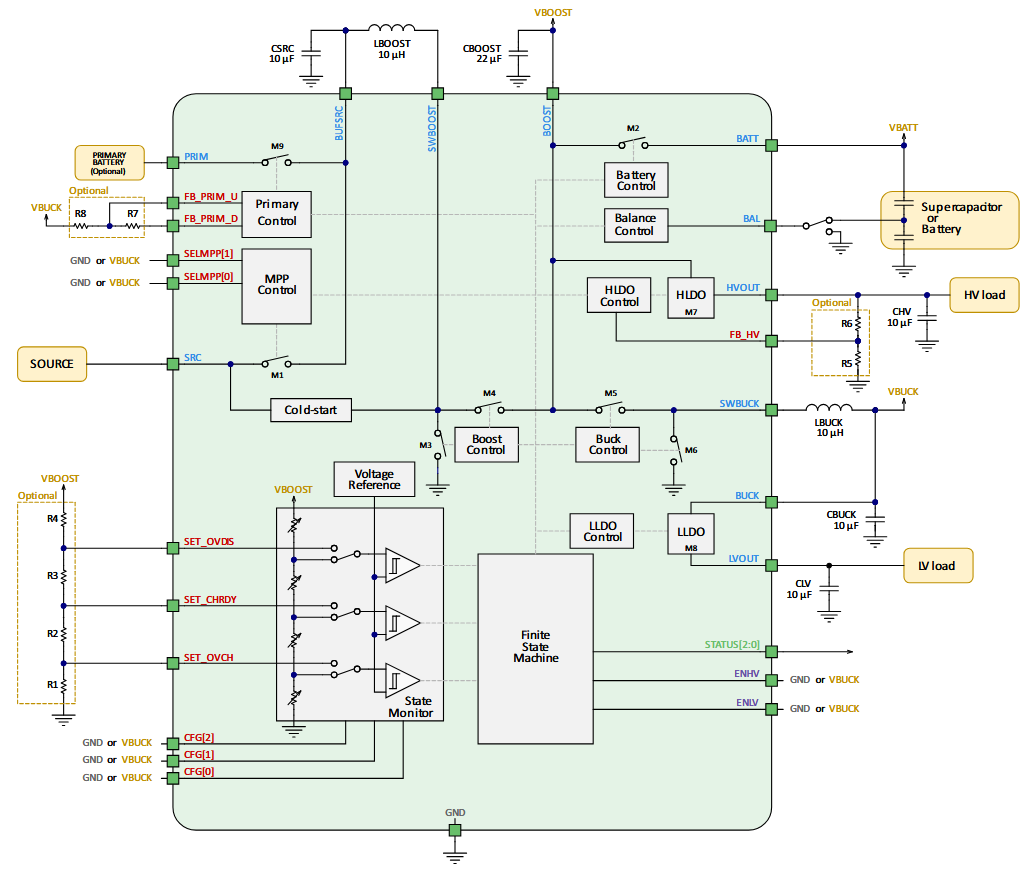
\includegraphics[width=0.65\textwidth]{imm/DS-AEM10941_VR_Block_Diagram.png}
    \caption{DS-AEM10941\_VR block diagram.}
    \label{fig:pmic_aem10941}
\end{figure}

\begin{table}[htbp]
    \centering
    \begin{tabular}{cccc}
        \toprule
        Symbol & Parameter & Range & Unit \\
        \midrule
        $V_{in}$ & Source input voltage & $0.05$-$5$ & V \\
        $V_{cs}$ & Source cold-start voltage & $0.38$ & V \\
        $V_{OC}$ & Open-circuit voltage tracked for MPP & $0.05$-$4.5$ & V \\
        \bottomrule
    \end{tabular}
    \caption{DS-AEM10941\_VR input stage.}
    \label{tab:pmic_aem10941_in}
\end{table}

The output voltage is regulated using a Buck converter with constant voltage (typ.\ $2.2\ \text{V}$) fed by the storage element. The IC additionally provides two \LDO{} outputs for low-noise, high-stability supplies.

\begin{table}[htbp]
    \centering
    \begin{threeparttable}
    \begin{tabular}{cccc}
        \toprule
        Symbol & Parameter & Range & Unit \\
        \midrule
        $V_\text{Buck}$ & Buck output voltage (typ.\ $2.2\ \text{V}$) & $2$-$2.5$ & V \\
        $V_{LV}$ & \LDO1 output voltage & $1.2$-$1.8$ & V \\
        $I_{LV}$ & \LDO1 output current & $0$-$20$ & mA \\
        $V_{HV}$ & \LDO2 output voltage & $1.8$-$4.1$\tnote{*} & V \\
        $I_{HV}$ & \LDO2 output current & $0$-$80$ & mA \\
        \bottomrule
    \end{tabular}
    \begin{tablenotes}
        \small
        \item[*] See the datasheet for additional details.
    \end{tablenotes}
    \end{threeparttable}
    \caption{DS-AEM10941\_VR output stage.}
    \label{tab:pmic_aem10941_out}
\end{table}

\subsection{bq25570}
\label{sec:pmic_bq25570}

\href{https://www.ti.com/lit/ds/symlink/bq25570.pdf}{Datasheet} \cite{tiBq25570Datasheet}

\begin{figure}[htbp]
    \centering
    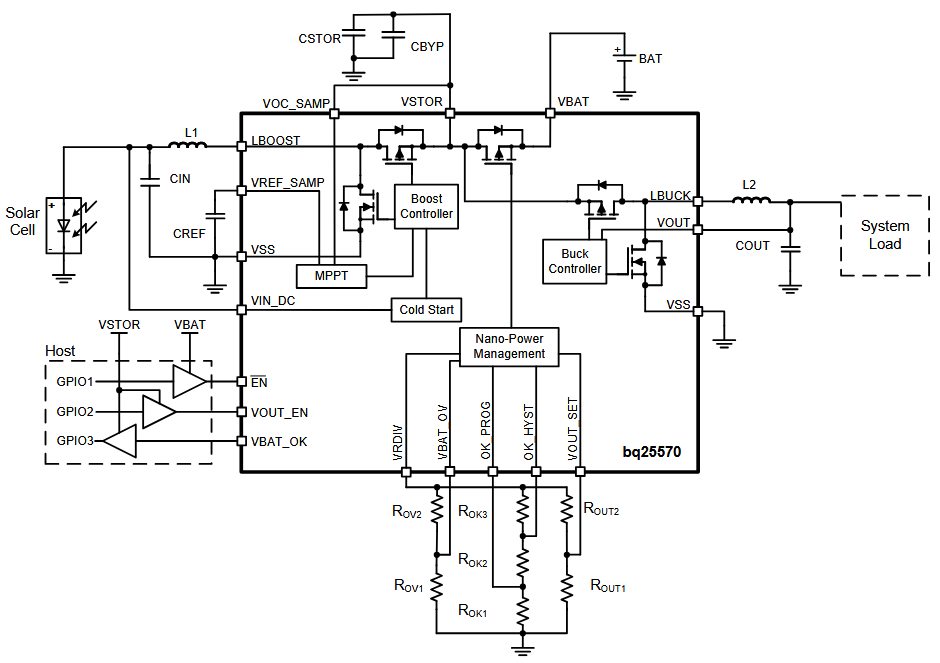
\includegraphics[width=0.7\textwidth]{imm/bq25570_Block_Diagram.png}
    \caption{bq25570 block diagram.}
    \label{fig:pmic_bq25570}
\end{figure}

\begin{table}[htbp]
    \centering
    \begin{tabular}{cccc}
        \toprule
        Symbol & Parameter & Range & Unit \\
        \midrule
        $V_{in}$ & Source input voltage & $0.1$-$5.1$ & V \\
        $V_{cs}$ & Source cold-start voltage & $0.6$ & V \\
        $V_{OC}$ & Open-circuit voltage tracked for MPP & $0.1$-$5.1$ & V \\
        \bottomrule
    \end{tabular}
    \caption{bq25570 input stage.}
    \label{tab:pmic_bq25570_in}
\end{table}

The output voltage is regulated with a Buck converter connected to the storage element.

\begin{table}[htbp]
    \centering
    \begin{tabular}{cccc}
        \toprule
        Symbol & Parameter & Range & Unit \\
        \midrule
        $V_\text{Buck}$ & Buck output voltage ($1.8\ \text{V}\pm2\%$) & $1.764$-$1.836$ & V \\
        $I_\text{Buck}$ & Buck output current & $83$-$110$ & mA \\
        \bottomrule
    \end{tabular}
    \caption{bq25570 output stage.}
    \label{tab:pmic_bq25570_out}
\end{table}

\subsection{SPV1050}
\label{sec:pmic_spv1050}

\href{https://www.st.com/resource/en/datasheet/spv1050.pdf}{Datasheet} \cite{stSpv1050Datasheet}

\begin{figure}[htbp]
    \centering
    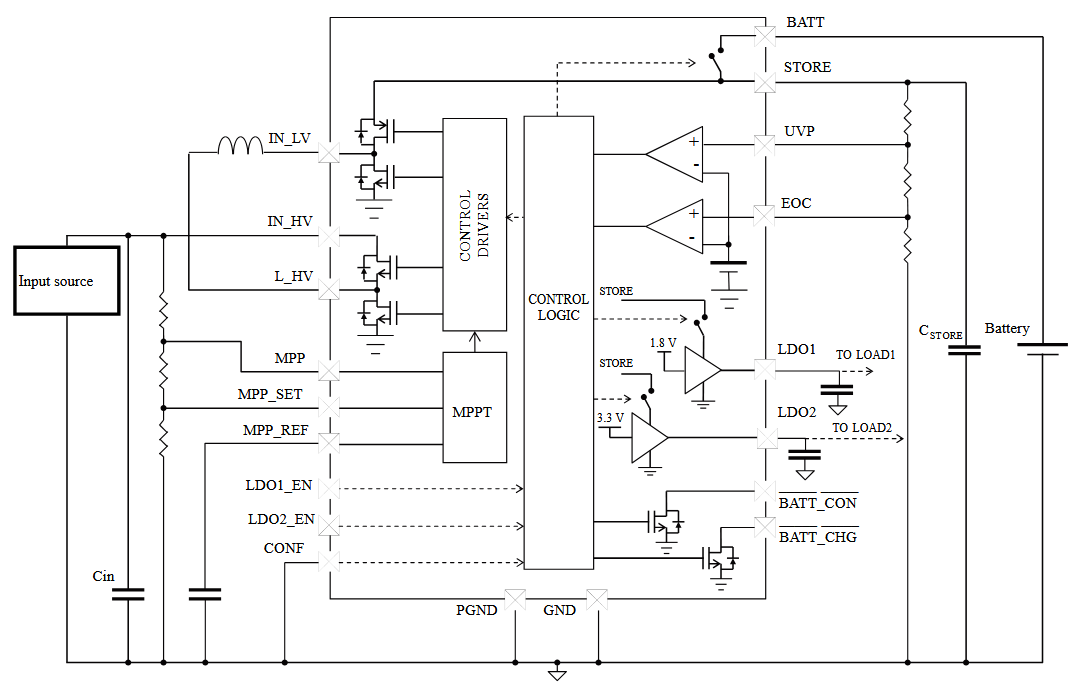
\includegraphics[width=0.65\textwidth]{imm/SPV1050_Block_Diagram.png}
    \caption{SPV1050 block diagram.}
    \label{fig:pmic_spv1050}
\end{figure}

The SPV1050 can be configured either as a Boost or as a Buck-Boost converter at its input stage; Table \ref{tab:pmic_spv1050_in} reports both.

\begin{table}[htbp]
    \centering
    \begin{tabular}{cccc}
        \toprule
        Symbol & Parameter & Range & Unit \\
        \midrule
        \multicolumn{4}{l}{\textit{Boost configuration}} \\
        $V_{in}$ & Source input voltage & $0.15$-$5.3$ & V \\
        $V_{cs}$ & Source cold-start voltage & $0.55$-$0.58$ & V \\
        $V_{OC}$ & Open-circuit voltage tracked for MPP & $0$-$5.3$ & V \\
        \addlinespace
        \multicolumn{4}{l}{\textit{Buck-Boost configuration}} \\
        $V_{in}$ & Source input voltage & $0.15$-$18$ & V \\
        $V_{cs}$ & Source cold-start voltage & $2.6$-$2.8$ & V \\
        $V_{OC}$ & Open-circuit voltage tracked for MPP & $0$-$18$ & V \\
        \bottomrule
    \end{tabular}
    \caption{SPV1050 input stage.}
    \label{tab:pmic_spv1050_in}
\end{table}

\begin{table}[htbp]
    \centering
    \begin{tabular}{cccc}
        \toprule
        Symbol & Parameter & Range & Unit \\
        \midrule
        $V_{LV}$ & \LDO1 output voltage & $1.8$ & V \\
        $I_{LV}$ & \LDO1 output current & $0$-$200$ & mA \\
        $V_{HV}$ & \LDO2 output voltage & $3.3$ & V \\
        $I_{HV}$ & \LDO2 output current & $0$-$200$ & mA \\
        \bottomrule
    \end{tabular}
    \caption{SPV1050 output stage.}
    \label{tab:pmic_spv1050_out}
\end{table}

\subsection{SPV1040}
\label{sec:pmic_spv1040}

\href{https://www.st.com/resource/en/datasheet/spv1040.pdf}{Datasheet} \cite{stSpv1040Datasheet}

\begin{figure}[htbp]
    \centering
    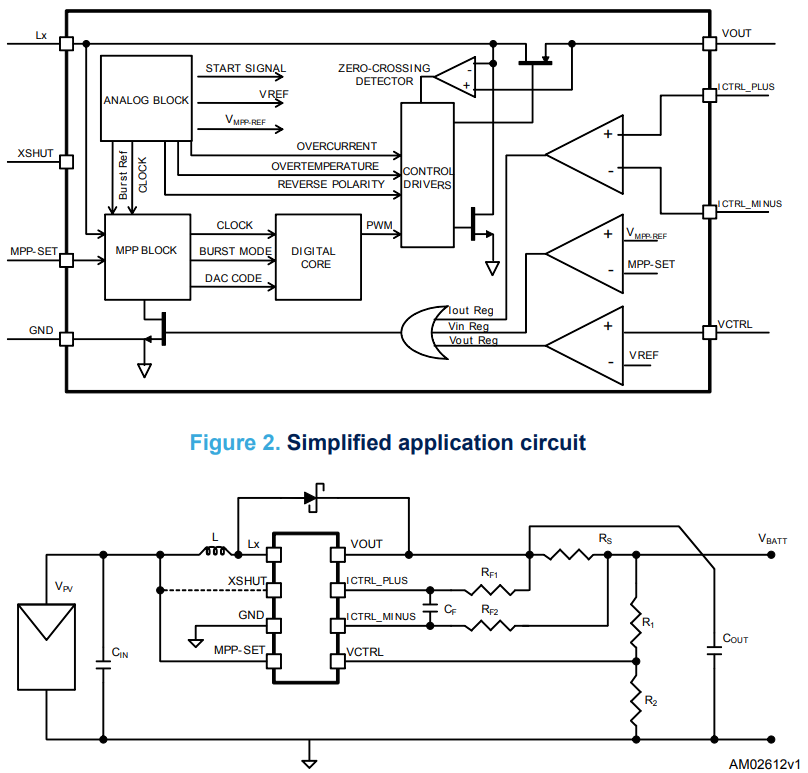
\includegraphics[width=0.65\textwidth]{imm/SPV1040_Block_Diagram.png}
    \caption{SPV1040 block diagram.}
    \label{fig:pmic_spv1040}
\end{figure}

\begin{table}[htbp]
    \centering
    \begin{tabular}{cccc}
        \toprule
        Symbol & Parameter & Range & Unit \\
        \midrule
        $V_{in}$ & Source input voltage & $0.3$-$5.5$ & V \\
        $V_{cs}$ & Source cold-start voltage & $0.8$-$2$ & V \\
        $V_{OC}$ & Open-circuit voltage tracked for MPP & $0$-$5.5$ & V \\
        \bottomrule
    \end{tabular}
    \caption{SPV1040 input stage.}
    \label{tab:pmic_spv1040_in}
\end{table}

No output-stage specification is available for this device from the source material used for this chapter.

\section{Compatibility Analysis}
\label{sec:pmic_compatibility}

Table \ref{tab:pmic_compatibility} compares each PMIC's input voltage range against the open-circuit voltage measured for each topology (Tables \ref{tab:pmic_ocv_star}-\ref{tab:pmic_ocv_nvc}), to identify over which part of the $100$-$400\ \text{rpm}$ tested range the two remain compatible. Since the delta connection's open-circuit voltage, including its ripple, never exceeds $3.755+0.017=3.772\ \text{V}$ and the NVC's never exceeds $3.20+0.639=3.839\ \text{V}$, both stay within the input range of every one of the six PMIC configurations across the whole tested speed range. The star connection, reaching $7.04+0.012=7.052\ \text{V}$ including its ripple at $400\ \text{rpm}$, exceeds the input range of four of the six configurations above a certain speed, listed in the table; only the SPV1050's Buck-Boost configuration, with its $18\ \text{V}$ upper limit, accommodates the star connection's open-circuit voltage across the entire tested range.

\begin{table}[htbp]
    \centering
    \begin{tabular}{lccc}
        \toprule
        PMIC (configuration) & $V_{in}$ range (V) & $V_{cs}$ (V) & Star connection \\
        \midrule
        DS-AEM13920\_VR & $0.120$-$4.6$ & $0.275$ & up to $250\ \text{rpm}$ \\
        DS-AEM10941\_VR & $0.05$-$5$ & $0.38$ & up to $250\ \text{rpm}$ \\
        bq25570 & $0.1$-$5.1$ & $0.6$ & up to $250\ \text{rpm}$ \\
        SPV1050 (Boost) & $0.15$-$5.3$ & $0.55$-$0.58$ & up to $250\ \text{rpm}$ \\
        SPV1050 (Buck-Boost) & $0.15$-$18$ & $2.6$-$2.8$ & full range \\
        SPV1040 & $0.3$-$5.5$ & $0.8$-$2$ & up to $300\ \text{rpm}$ \\
        \bottomrule
    \end{tabular}
    \caption{Input-voltage compatibility of each PMIC configuration with the star connection over the $100$-$400\ \text{rpm}$ tested range. The delta connection and the NVC are compatible with every configuration across the full range, and are omitted from the table.}
    \label{tab:pmic_compatibility}
\end{table}

Cold-start capability follows a different pattern, since it is set by the source cold-start voltage $V_{cs}$ rather than the upper end of the input range, and must be met already at the lowest speed the harvester is expected to start from, $100\ \text{rpm}$. Against the $V_{cs}$ values in Table \ref{tab:pmic_compatibility}, all three topologies exceed the cold-start threshold of the first four configurations (at most $0.6\ \text{V}$) already at $100\ \text{rpm}$, where the lowest of the three open-circuit voltages, the delta connection's, is still $1.00\ \text{V}$. The much higher threshold of the SPV1050's Buck-Boost configuration ($2.6$-$2.8\ \text{V}$) is not met by any topology at $100\ \text{rpm}$: the star connection crosses it by $150\ \text{rpm}$ ($2.83\ \text{V}$), the NVC sits at the edge of the range already at $100\ \text{rpm}$ ($2.70\ \text{V}$) and clears it by $150\ \text{rpm}$ ($3.05\ \text{V}$), and the delta connection only clears it by $300\ \text{rpm}$ ($2.825\ \text{V}$). The SPV1040's threshold ($0.8$-$2\ \text{V}$) sits closer to the three topologies' voltages at $100\ \text{rpm}$: the star connection is already at the top of the range ($1.98\ \text{V}$), the NVC is above it ($2.70\ \text{V}$), and the delta connection sits within the lower half of the range ($1.00\ \text{V}$), only clearing its upper bound between $200$ and $250\ \text{rpm}$.

Overall, the delta connection and the NVC can be paired with any of the five PMICs considered without additional input protection, cold-starting at the lowest speed tested for four of the six configurations. The star connection delivers the highest open-circuit voltage, and, as Chapters \ref{ch:measurements} and \ref{ch:comparison} show, the highest output power at higher speeds. To use it safely above $250$-$300\ \text{rpm}$, though, it would need either the wide-range SPV1050 Buck-Boost configuration, or a clamp added in front of a narrower-range device to protect its input.
